\chapter{Experiments}

%Leave description of DECAL concept to DECAL chapter but mention it as one of the ECAL alternatives here

There are many possible designs for future lepton colliders \cite{Lipton:2012du,Koratzinos:2014cla} however here we focus on the two most developed projects, \ac{CLIC} and \ac{ILC}. Both projects are linear colliders which propose using electron-positron collisions and were founded over twenty years ago, though \ac{ILC} is currently the more mature design of the two. We will also discuss the detectors proposed for both experiments. \ac{ILC} currently has two detector concepts being developed, \ac{ILD} and \ac{SiD}, which will be operated in a 'push-pull' scheme in which both detectors are placed on a signle platform that is periodically moved to alternate which detector is placed in the path of the beams. This is necessary as there is only one interaction point at a linear collider. Having two detectors has the advantage that any results made with one detector can be verified with the second to help reduce any systematic bias from either machine, however it comes with the penalty that each detector will only be able to take data half of the time and the process of moving the detectors in and out is lengthy (INSERT NUMBERS) resulting in additional deadtime for the experiment. \ac{CLIC} intends to operate with only one detector, a variation of the \ac{ILD} developed for \ac{ILC}, adapted for the different beam conditions present at CLIC. 

\section{ILC}

The ILC (\reffig{Fig:ILC}) is a proposed experiment consisting of a 31km ${e^+e^-}$ collider to be built in Kitakami in the northern region of Japan. The current construction schedule predicts the experiment will be finished in the (NUMBERS) with a cost of the order \pounds6 billion and will run for approximately 20 years. However, until funding is secured for the experiment this is just an estimate. The \ac{ILC} \ac{TDR} \cite{ILCTDR} was released in 2013 and gives a full description of the experiments' baseline design. While the \ac{TDR} is highly detailed, because the experiment is still under development it is possible that some of the information contained within it will become outdated and change before construction takes place. For simplicity any figures given in this section can be assumed to be taken from the \ac{TDR} unless otherwise stated.

\begin{figure}
  \centering
  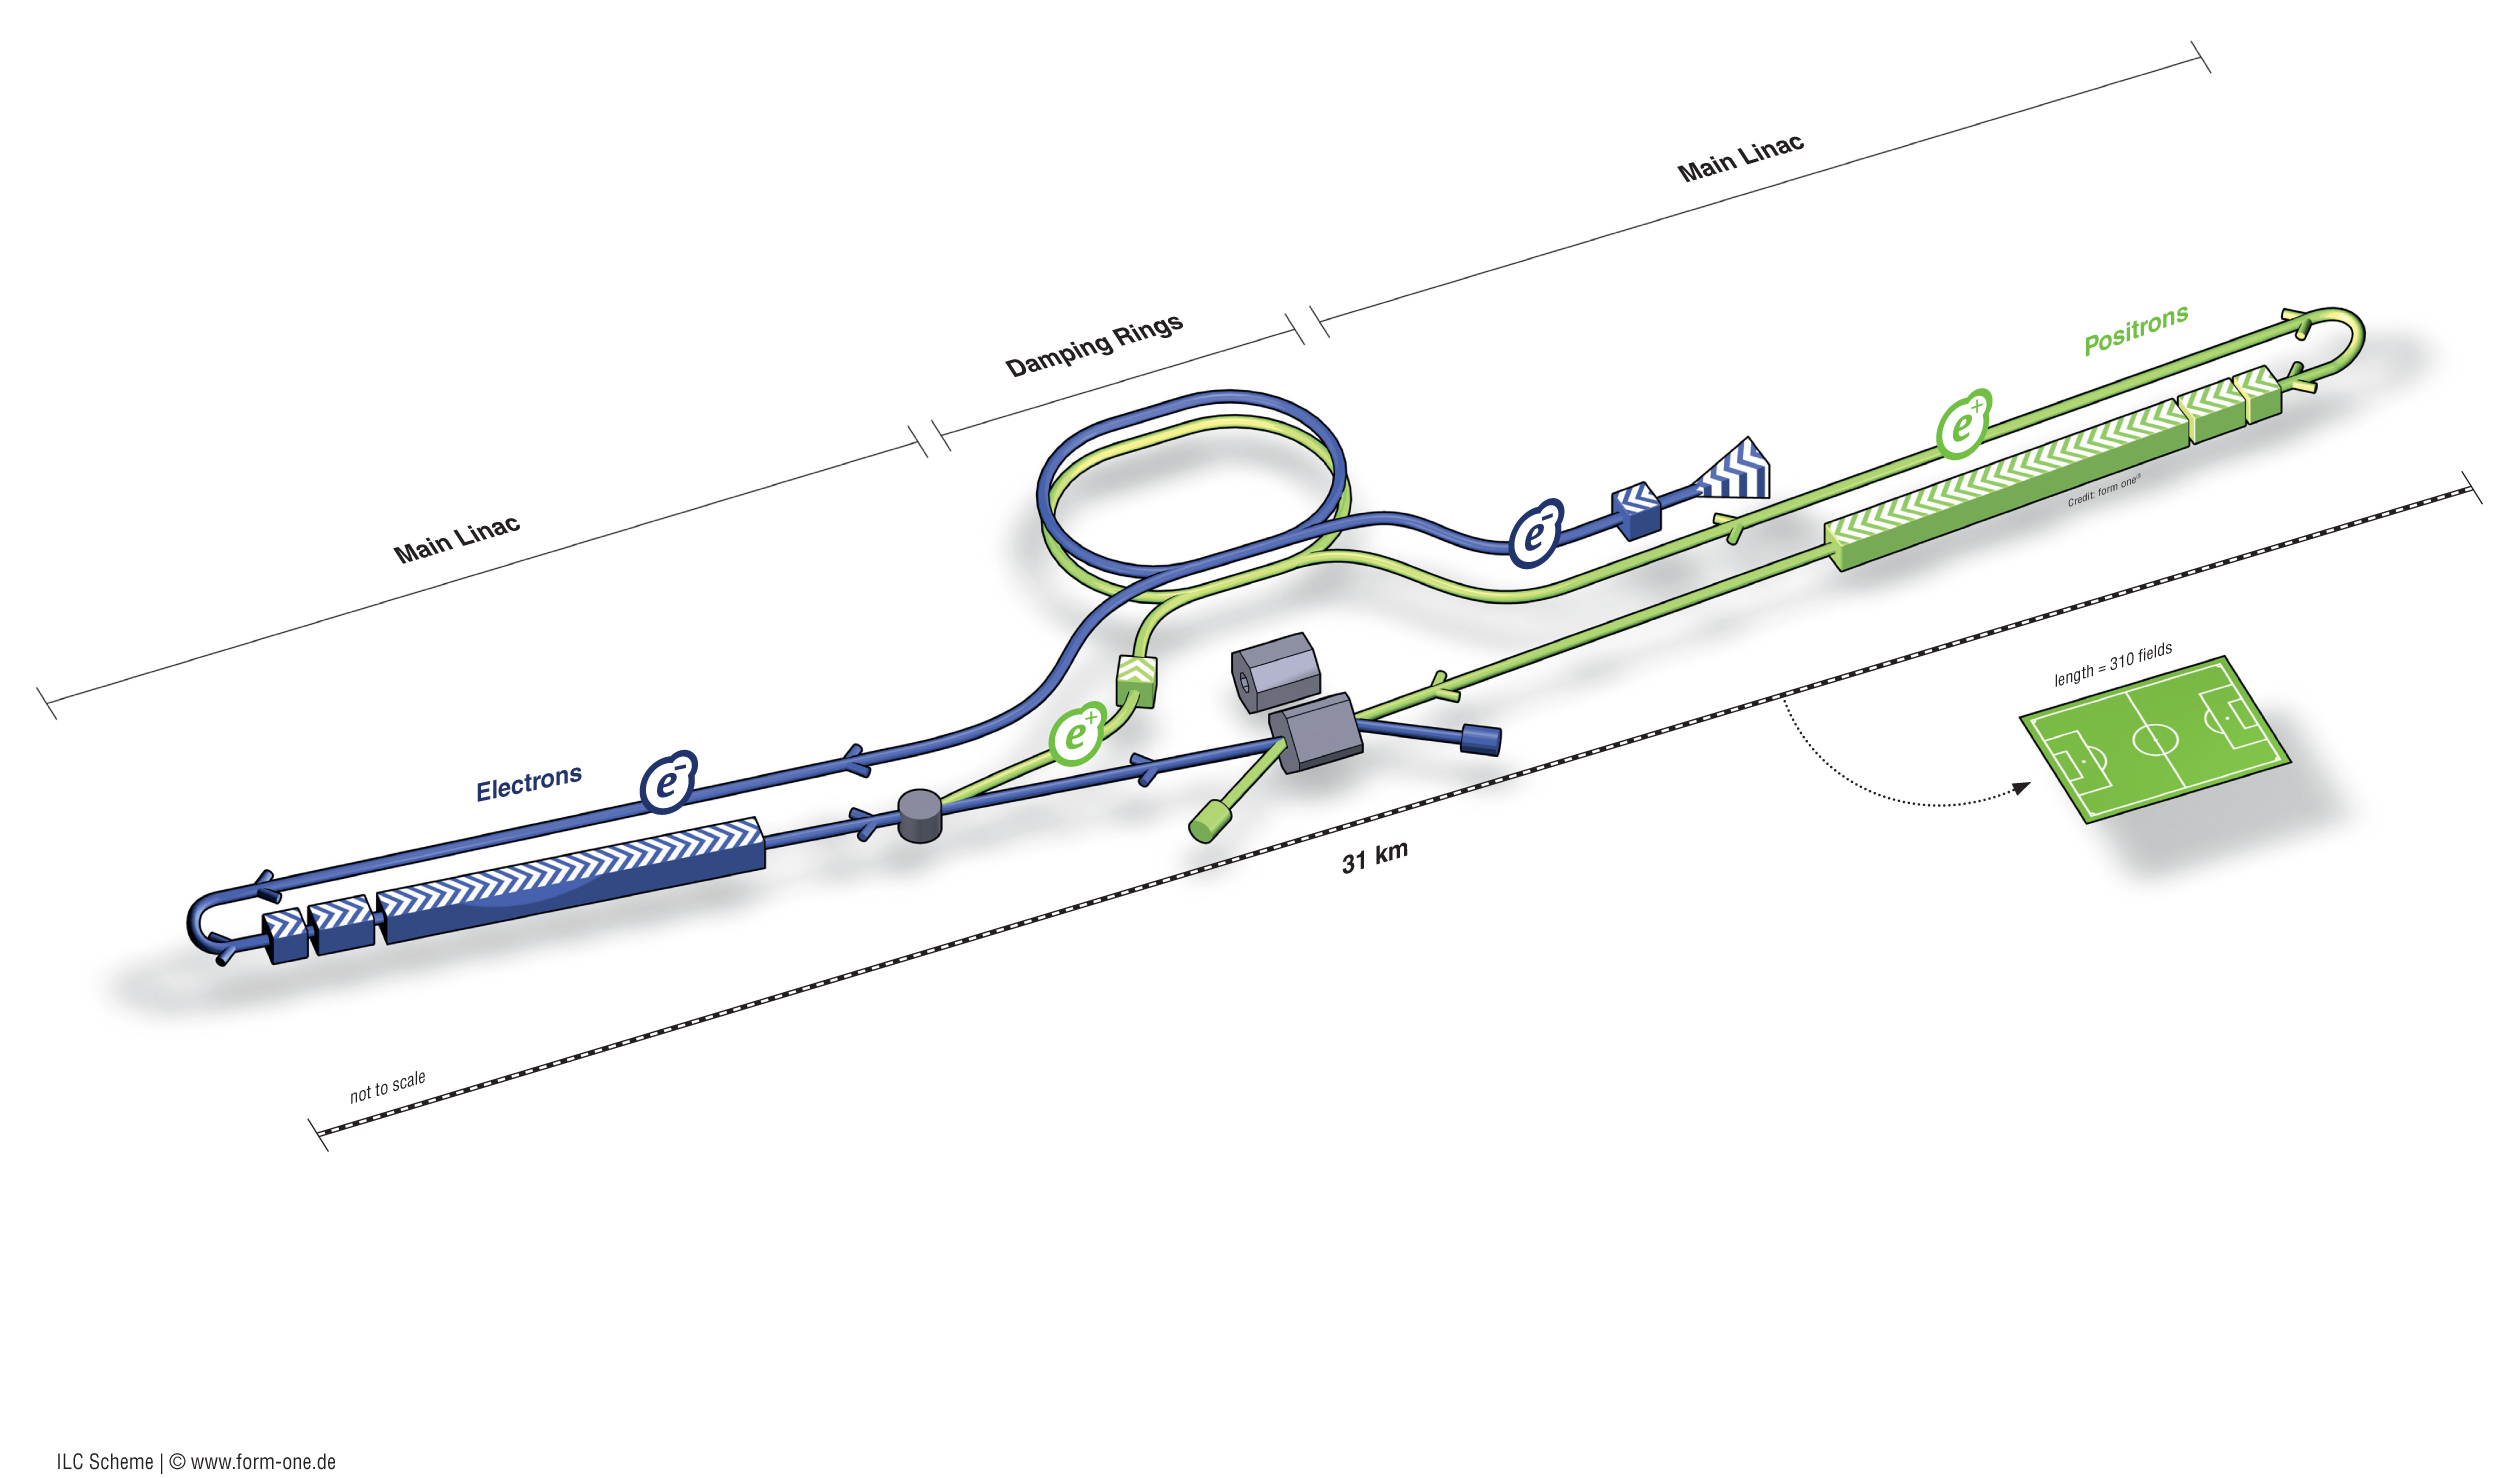
\includegraphics[width=0.75\textwidth,height=10cm,keepaspectratio]{Experiments/fig/ILC}
  \caption[The ILC Experiment]{The \ac{ILC} Collider (from \cite{ILCTDR})}
  \label{Fig:ILC}
\end{figure}

\subsection{Energy Staging}
CHECK ALL THESE NUMBERS!! Staging has changed!!!!

The \ac{ILC} will first be built with a maximum collision energy capability of 500GeV but with the potential for a later upgrade to 1TeV which would require doubling the length of the machine to 62km. The decision of whether the 1TeV upgrade is necessary will largely be determined by the results of the \ac{LHC} experiments; if any new physics is discovered above 500GeV then the 1TeV upgrade could be essential to characterise them. Assuming the 1TeV upgrade is realised the energy staging will be as described below.

The first three years will involve the ILC running at an energy of 250GeV and taking 250fb${^{-1}}$ of data. The main aim at this stage will be to measure the Higgs mass and ZH cross section from the Higgsstrahlung process described above. At this energy the experiment will have little sensitivity to the Higgs-WW coupling.

For the following three years, the collider will then run at 500GeV and will accrue a further 500fb${^{-1}}$ of data. The main aims here will be to measure the H-WW coupling, the total Higgs width and the absolute Higgs couplings to fermions. At this energy, measurements of top physics will also be possible including the top forward backward asymmetry. Outside of the Higgs, the top quark is perhaps the least well measured of the standard model particles and so provides another area in which to look for deviations from the standard model predictions.

After this there will be the upgrade to 1TeV followed by another three years of data taking accumulating 1000fb${^{-1}}$ of data. The aim of running at this high energy will be to search for new particles such as dark matter candidates and supersymmetric particles. If one of these (or something entirely new) has already been discovered at the \ac{LHC} then the choice of 1TeV might be scaled down to somewhere between 500GeV and 1TeV to match the scale of the newly discovered physics.

After this the collider will undergo a high luminosity upgrade and will run at the same energies for the same time periods for another 9 years but instead accruing 900, 1100 and 1500${fb^{-1}}$ at the respective energies. This will allow for a further increase in the precision of all measurements taken during the lower luminosity run.
While the \ac{TDR} proposes the above run scheme for the \ac{ILC} there is still debate about what energies should be used with arguments being made for running at 90GeV (the Z mass) to gain precision measurements of the Z boson and 350GeV (the top production threshold) to better measure the properties of the top quark.

\subsection{Beam Production, Acceleration and Focusing}
\label{ILC:BEAM}

\begin{figure}
  \centering
  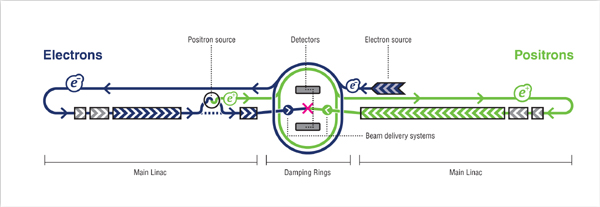
\includegraphics[width=0.75\textwidth,height=10cm,keepaspectratio]{Experiments/fig/ILC_Simplified}
  \caption[Schematic Of The ILC]{A simplified schematic of the ILC}
  \label{Fig:ILCsimple}
\end{figure}

A simplified schematic of the \ac{ILC} accelerating structure is shown above in diagram \reffig{Fig:ILCsimple}. The first stage of the acceleration process is the production of electrons. This is done using the photoelectric effect by firing photons onto a GaAs target to produce photoelectrons. These electrons then enter a 3.2km long damping ring which accelerates the beam up to 15GeV. The primary purpose of the damping ring is to produce a homogeneous beam of electrons with uniform energy and momentum. After the damping ring the electrons enter into a two stage bunch compressor which separates the electron beam into ${\sim}$1300 bunches, each containing ${2\times10^{10}}$ electrons, with each bunch being separated by 554ns giving a beam pulse length of 730${\mu}$s. The overall intended collision rate of these pulses is 5Hz, which means that the duration for collisions is less than 1\% of the collision rate. This has important consequences for the detector design as it means the detectors have a large period of time in which to relax after events. As the detectors do not need to be on for 99\% of the time, it is considerably easier to cool them meaning the material budget for the cooling systems within them can be greatly reduced. Following the bunch compression the electrons enter the main 11km linac where they are accelerated up to the nominal beam energy using 7,400 1.3GHz superconducting niobium \ac{RF} cavities (see \reffig{Fig:cavity}) 

\begin{figure}
  \centering
  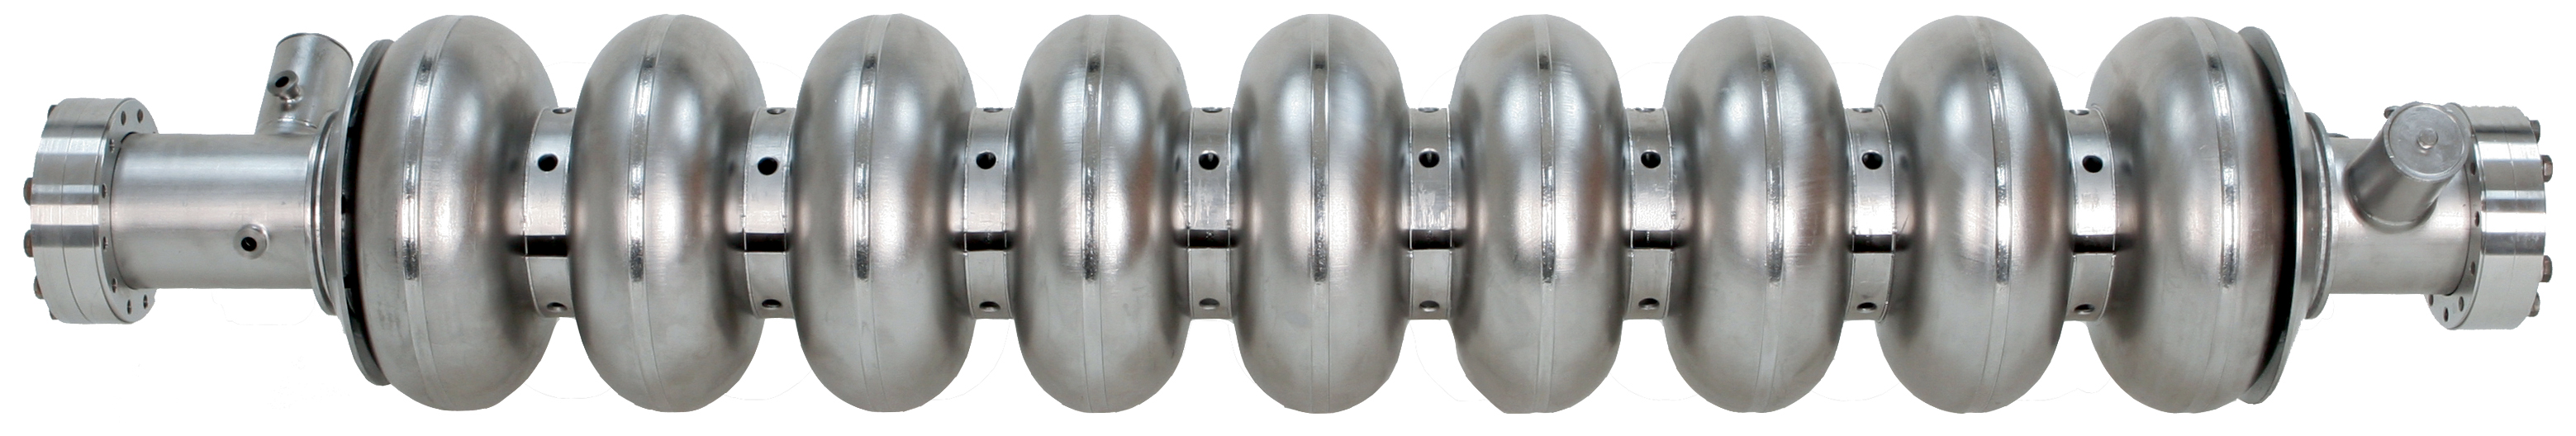
\includegraphics[width=0.75\textwidth,height=10cm,keepaspectratio]{Experiments/fig/Cavity}
  \caption[Superconducting Cavities For The ILC]{A 1.3GHz Superconducting Niobium Radio Frequency Cavity \cite{ILCTDR}}
  \label{Fig:cavity}
\end{figure}
The \ac{RF} cavities are kept at a temperature of 2K and act to produce an average accelerating gradient of up to 31.5MV/m (14.7MV/m for the 250GeV stage.)  The final stage before the collision is the \ac{BDS} which primarily acts to compress the beam into a ribbon shape with a cross-section of 7.7 x 729.0 nm while also handling the beam monitoring. The ribbon shape acts to reduce the \ac{BS} radiation described earlier (see \refsec{benefits}) while giving a small enough cross-section that the \ac{IP} of the collision can be well known. Following the \ac{BDS} the beam finally enters the detector and collides with the oppposing positron beam at a crossing angle of 14mrad then exits into the beam dump system which quenches what is left of the beam.

\subsection{Positron Production}
Positrons are produced at the \ac{ILC} by tapping off energy from the electron beam after it has been accelerated by the main linac. The electron beam is passed through an undulator which causes the electrons to emit synchrotron radiation in the form of 10-30MeV photons by forcing the beam to take a rapidly varying path in the transverse plane to it's direction of motion. The resulting photons are then separated from the electron beam and are collided with a Titanium alloy target to produce electron positron pairs. The electrons and positrons are then separated- the electrons are dumped while the positrons are then passed into a damping ring and undergo all the same stages of acceleration and shaping as described above for the electrons.

\section{CLIC}
AGAIN CHECK ALL NUMBERS!!!!

\begin{figure}
  \centering
  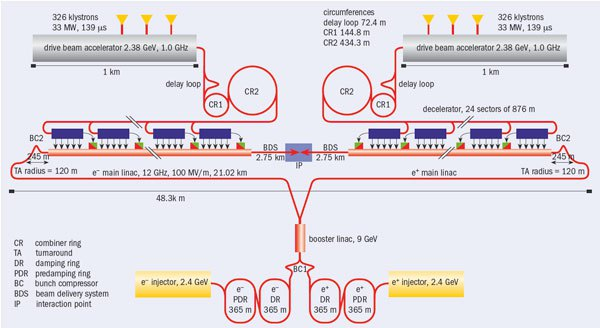
\includegraphics[width=0.75\textwidth,height=10cm,keepaspectratio]{Experiments/fig/clic}
  \caption[The CLIC Experiment]{The CLIC Collider. Image taken from CLIC Conceptual Desgin Report\cite{CDR}}
  \label{Fig:CLIC}
\end{figure}
\ac{CLIC} is an experiment based at CERN which proposes the building of a 42km accelerator at the main CERN site in Geneva (\reffig{Fig:CLIC}.) Despite being named as “compact”, \ac{CLIC} is actually longer than the initial 500GeV \ac{ILC}. The reason for this naming is that \ac{CLIC} has a much higher accelerating gradient (100MeV/m) compared to ILC and so provides a much higher energy per length. The expected build date for \ac{CLIC} is still relatively uncertain though is likely to be no earlier than 2030 as the accelerating technology required for \ac{CLIC} is less developed than for \ac{ILC}. This difference in the maturity of the two experiments can be seen from the fact that the \ac{ILC} has released its \ac{TDR} while the most comprehensive document for the CLIC project is still its \ac{CDR} \cite{CDR}. Updates on this document have been provided in the New Baseline Report \cite{UpdatedCLICBaseline} released  in (NUMBER YEAR) and any details specified here can be assumed to come from these two documents. 

Overall the design for \ac{CLIC} is relatively similar in layout to the \ac{ILC} but with a few changes. Positron production at \ac{CLIC} is done completely independently from the main electron beam, though they are still produced via the same mechanism as before. The \ac{BDS} still compresses the beam to give it a small cross-section but the beam is no longer shaped into a ribbon shape- this is why photon radiation is a more significant problem at \ac{CLIC}. The collision rate at \ac{CLIC} is significantly higher as it aims to be a high luminosity device- the collision rate will be 50Hz with 354 bunches per pulse with a separation of just 0.5ns. This means that CLIC will have a significantly higher duty cycle which will make cooling of the detectors harder and will give the detectors less time to relax after events. The most significant differences however are the energy staging and the acceleration technology used at \ac{CLIC}.

\subsection{Energy Staging}
UPDATE STAGING!!

CLIC will operate at three energy stages- 380GeV, 1.5TeV and 3TeV collecting 500${fb^{-1}}$, 1.5${ab^{-1}}$ and 2${ab^{-1}}$ of data respectively. During the running of the 380~GeV energy stage, construction of the 1.5~TeV structure will be carried out (and so on for the 1.4TeV and 3TeV scales) so as to reduce the waiting time between successive energy stages. 

The 380GeV energy scale is chosen as it is above the \ttbar production threshold and provides a significant cross section for many channels involving the top quark. This is stage is also supplemented by a series of 10 measurements around the \ttbar threshold taking 10${fb^{-1}}$ each with the aim of measuring the top mass and width from the line shape of the \ttbar production cross section at threshold. The 380~GeV stage will also be used to provide measurements of the higgs boson similar to those performed at \ac{ILC} during it's two lower energy stages.

The 1.4TeV energy stage provides the ability to further study the top and higgs in more detail with several new channels becoming significant e.g top yukawaw coupling, higgs self coupling while the 3~TeV stage pushes the energy frontier allowing the possibility of direct detection of new physics at the multi-TeV scale. The choice of 3~TeV is based upon certain models of supersymmetry which predict new particles to exist at this energy (see \ref{SuperSym}.)

For clarification it should be stated that for many years the proposed scheme for CLIC was actually to operate at 350~GeV, 1.4~TeV and 3~TeV. As such, many of the studies performed by CLIC still quote these numbers in cases where the result is expected to be unchanged when switiching to the new baseline. The main justifications for the new baseline is to improve prospects for certain top quark studies performed in the low energy stage.

\begin{figure}
  \centering
  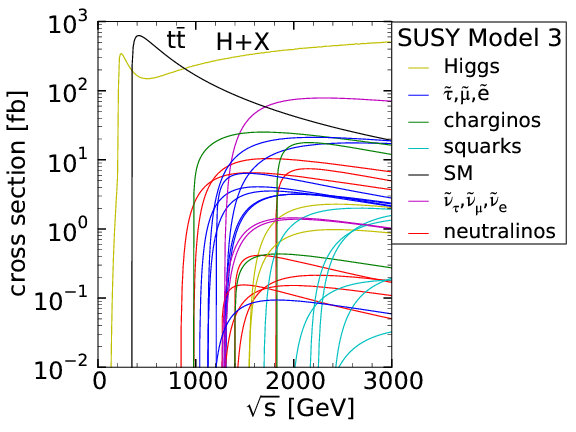
\includegraphics[width=0.75\textwidth,height=10cm,keepaspectratio]{Experiments/fig/clicSS}
  \caption[Cross Sections For Super Symmetric Processes]{Cross sections for production of various super symmetric particles at an ${e^+e^-}$ collider as a function of centre of mass energy.}
  \label{Fig:SuperSym}
\end{figure}

\subsection{Acceleration Technology}
Unlike \ac{ILC}, the acceleration technology will not be superconducting and will use two beams of electrons-- referred to as the main beam and the drive beam-- rather than just one main accelerated beam. The drive beam is accelerated using standard accelerating technology (Klystrons) as in \ac{ILC} to accelerate bunches of electrons to 2.75GeV. These bunches then enter a series of delay/control rings which are designed such that the electrons within them get combined with the new electrons being added from the drive beam accelerator to build up a large number of low energy electrons which combined carry a large amount of energy. The energy from this beam is then used to drive the main beam. This is done by rapidly decelerating the drive beam electrons down to 10\% of their initial energy and using the lost energy (emitted as photons) to accelerate the smaller number of electrons in the main beam resulting in a sudden rapid acceleration. The main beam is then used for the collisions. Overall the result is that the machine is simply converting a high current, low energy beam of electrons into a low current, high energy beam. This approach allows for very high accelerating gradients but has the disadvantage that in approximately 1\% of events the sudden input of energy from the drive beam can cause electrical breakdowns in the main accelerator, which disrupt the alignment and structure of the main beam.


\section{Detectors}
The \ac{ILC} has been designed with the intention that it will have two unique detectors so that results can be validated by cross-checking between the two detectors. However, because \ac{ILC} is a linear collider it is only feasible to have one interaction point and as a result the beam time will have to be shared between the detectors. This will be done using a 'push-pull' design in which both detectors are placed on a single platform at the interaction point which can be moved back and forth to position the desired detector in the path of the beams. While having two detectors is certainly desirable as it allows us to get two independent sets of results for the collider and allows us to still take results when one of the detectors requires maintenance, it also has disadvantages as it means an increase in the dead time of the machine (as swapping the detectors is a slow process taking several days which will be done multiple times a year) and an increase in the cost of the experiment. As a result the possibility of using only one detector is still being considered as a potential option. The possibility of splitting the main beam and having two IPs is also being proposed so that both detectors could be used simultaneously however this would be expensive as extra tunnels would have to be built to accomodate this and there would also be a reduction in the beam quality as splitting the beam would produce synchotron radiation.
\subsection{ILD}
\begin{figure}
  \centering
  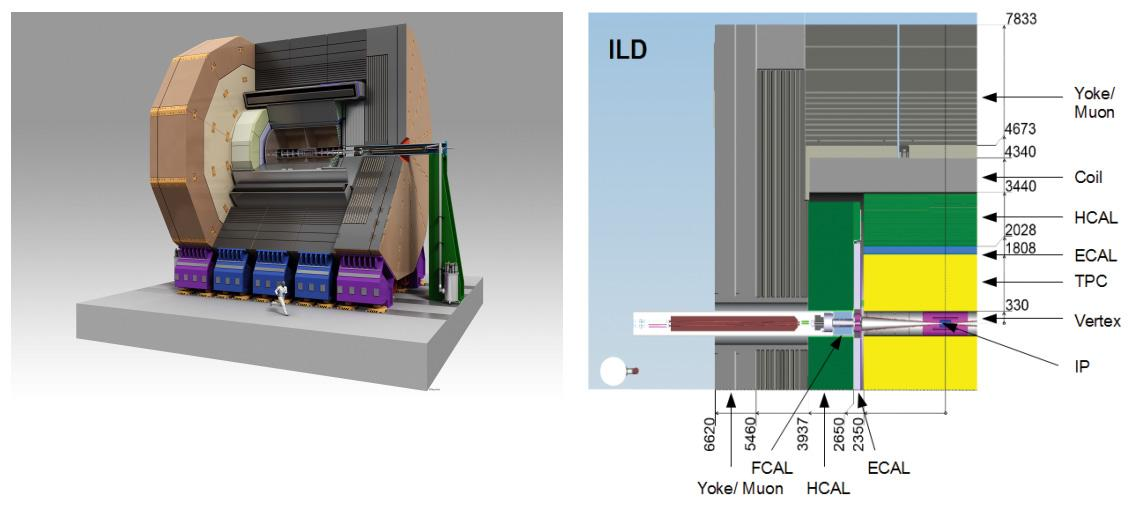
\includegraphics[width=0.95\textwidth,keepaspectratio]{Experiments/fig/ILD}
  \caption[ILD Detector]{The International Large Detector Concept (left). Schematic of the ILD showing the key components in a one-quarter view of a vertical section of the detector (right). \cite{ILCTDR}}
  \label{Fig:ILD}
\end{figure}
The ILD (shown in \reffig{Fig:ILD}) is a general purpose detector which is cylindrical in design with radius 8m and length 14m. The different sub-detectors are arranged in a concentric manner in the main barrel of the detector, and are positioned with the vertexing technology closest to the beamline, followed by trackers, then electromagnetic and hadronic calorimeters, then the magnetic field coils and finally muon tail catchers. The detector has two endcaps at each end of the barrel creating a hermetic seal. Because many of the physics processes at \ac{ILC} involve Z and W bosons, one of the main performance requirements is the ability to distinguish between the two particles which means achieving a 3-4\% uncertainty in the energy of 100GeV jets and a ${\delta p}$/${p^2}$ (where $p$ is the momentum of a charged particle) of ${5\times10^{-5} (GeV/c)^{-1}}$. All specifications for the detector can be found in the \ac{ILD} Letter of Intent \cite{ILD}. Here we will give a brief overview of the key components and their functions.

\subsubsection{Vertexing}
The vertexing technology is used to gain information about heavier particles such as b-quarks which have very short lifetimes ($\sim$10$^{-12}$s) and so decay close to the beamline before they can reach the trackers or calorimeters. As such, the vertexers are placed extremely close to the beamline and work by looking for displaced vertices from the initial \ac{IP} which correspond to the point at which the heavy flavour paricles decayed. Due to their proximity to the beam line it is always necessary for the vertex detectors to be very radiation hard as they are exposed to stray high energy particles from the beam. The vertexers also act as trackers for short lived particles that fail to reach the main trackers and so are required to be highly granular to separate particles that have had very little time to spread out since the \ac{IP}. The design for the vertex detectors is yet to be finalised as there are numerous competing technologies under consideration but it is expected to consist of either 3 or 5 cylinders of sensors starting at a radius of $r=15$mm from the beamline.

\subsubsection{Tracking}
Tracking at the \ac{ILD} uses a \ac{TPC}. This is a large gas filled cylinder with an electric field across it and readout electronics at each end of the cylinder. As particles pass through the gas, they ionize it producing charged particles. The electric field then causes these particles to drift to each end of the detector where they are collected by the electronics. By measuring the position and time at which the charged particles arrive, the track of the original ionizing particle can be reconstructed. A magnetic field is also generated across the chamber to deflect the charged particles so that the momentum and charge of the particle can be estimated. The magnetic field used in the ILD is a 3.5T coil placed outside the calorimeters to minimize the material budget in front of the calorimeters. To gain extra precision on the entry and exit points of the \ac{TPC}, the chamber has two silicon detector layers referred to as the \ac{SIT} and \ac{SET} positioned  immediately before (r=165mm) and after (r=1833mm) the \ac{TPC} which give two high spatial resolution points for the entrance and exit points of particles. These high spatial resolution points are particularly useful for reconstructing individual particles within jets using the Pandora \ac{PFA} (see \refsec{Pandora}.)

\subsubsection{Calorimetry}

The function of calorimeters is to measure the energy of particles. The ILD uses sampling calorimeters which work by having alternating layers of a dense absorber material that destroy the incoming particle causing it to shower into lower energy particles and active sensor materials which collect the low energy particles and convert them into an electrical signal. The calorimeters are split into electromagnetic and hadronic sections in which the absorbing material is chosen to interact mainly with particles through electromagnetic or strong interactions respectively. In practice this means the \ac{ECAL} mainly detects electrons and photons while the \ac{HCAL} mainly detects hadrons such as pions. Neutral hadrons are recorded exclusively in the \ac{HCAL}.

The ILD ECAL is a highly granular calorimeter poitioned at r=1847mm and consists of 30 active layers separated by layers of tungsten which acts as the absorbing material. The structure of the \ac{ECAL} is shown in \reffig{Fig:ECAL}. The choice of active material is yet to be made though the two leading techologies are silicon scintillators or pixels. The scintillator form of the technology uses 10x45mm strips which would be rotated by 90${^o}$ in each successive layer to produce an effective cell size of 10x10mm with photomultipliers attached to each strip for readout. This form of the technology is considerably cheaper but has a lower performance and relies on algorithms accurately correlating hits in successive layers to produce the effective 10x10mm cell size. The pixel form of the technology simply uses 5mm or 10mm square silicon pixels directly connected to the readout electonics. This is more expensive but produces more consistent results.

\begin{figure}[h]
  \centering
  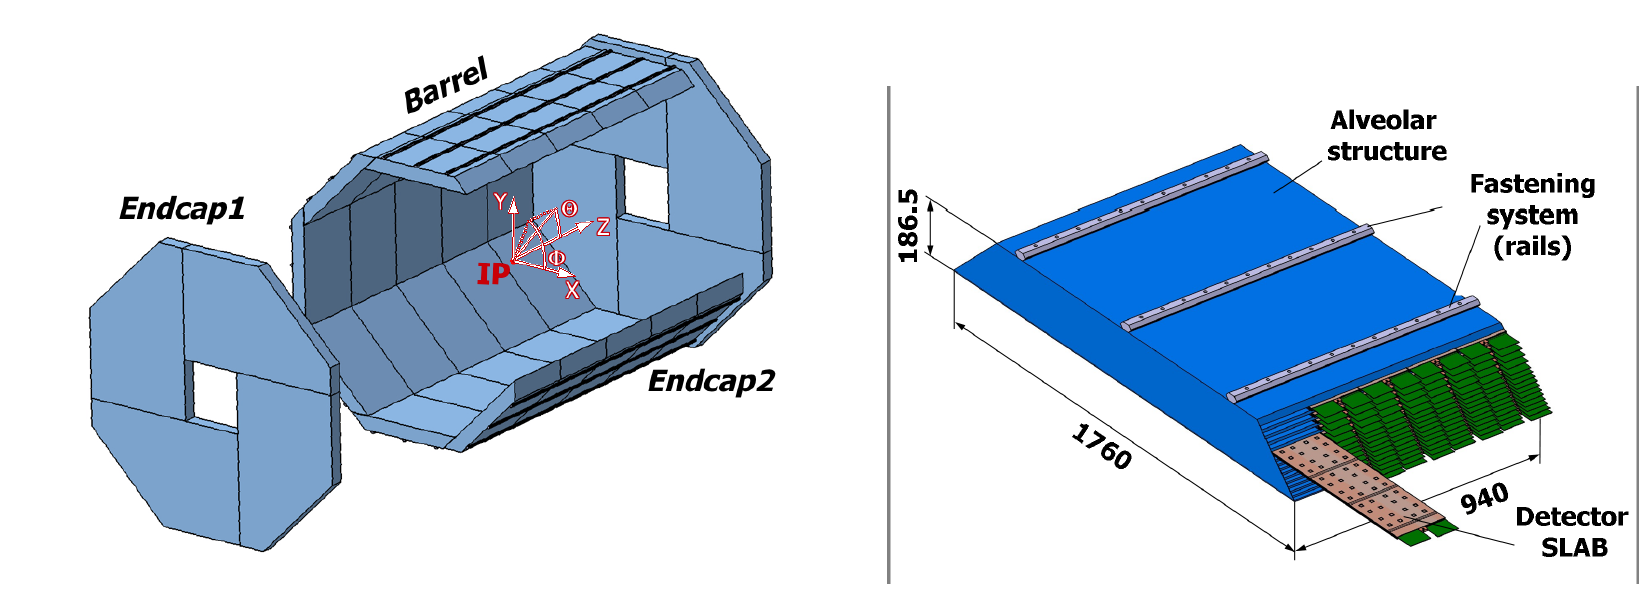
\includegraphics[width=0.95\textwidth,keepaspectratio]{Experiments/fig/ecalstructure} %aw replace image with higher quality version
  \caption[ECAL Structure]{The Overall ILD Structure (left) and one individual module (right).The ECAL is made up 40 modules, each containing 30 detector slabs. The modules are combined into groups of 5 referred to as a stave whih extend along the full length of the barrel. There are then 8 of these stave arranged in a circle to create the circumference of the barrel \cite{ILD}.}
  \label{Fig:ECAL}
\end{figure}

Later on (see \refsec{Sect:DECAL}) we will discuss our work on developing an alternative form of the silicon pixel technology with a cell size of 50x50${\mu}$m which acts as a digital machine and purely counts the number of particles absorbed in the active medium from the showering in the absorber and deduces the energy of the original particle from this.  This form of the technology has already begun to be studied \cite{2011JInst...6.5009B}. It is expected to be cheaper than the standard silicon pixel tehnology and has already been shown to produce no significant decrease in performance.

The \ac{HCAL} is immediately outside the ECAL at r=2058mm and has a similar overall modular structure. The HCAL uses stainless steel as an absorbing medium combined with scintillators and Silicon PhotoMultipliers. Again both digital and analogue variations are available with the analogue using 3x3cm cells and the digital 1x1cm. The relative performance of each technology is still being evaluated to see if there is any degredation in the performance when using the digital variation.

\subsubsection{Muon Detection}
Muon detection is perhaps the easiest process to perform at the ILC. Because the signal events at the ILC are clean with few high energy particles, few particles other than muons are capable of penetrating through the inner detector layers and the coil generating the magnetic field. As a result the muon detetors are produced by instrumenting the return yolk (r=4424) that already surrounds the detector to contain the magnetic field. The number of muons produced in an event is also relatively small which means that the cell size for the muon detectors can be moderately large without the risk of multiple occupancy. The instrumentation is done by placing 10 layers of resistive plate chambers into the return yolk with strip sizes of the order 3-4cm. This system is sufficient for accurately detecting muons and contributing to the measurement of their momentum.

\subsection{SiD}

\begin{figure}
  \centering
  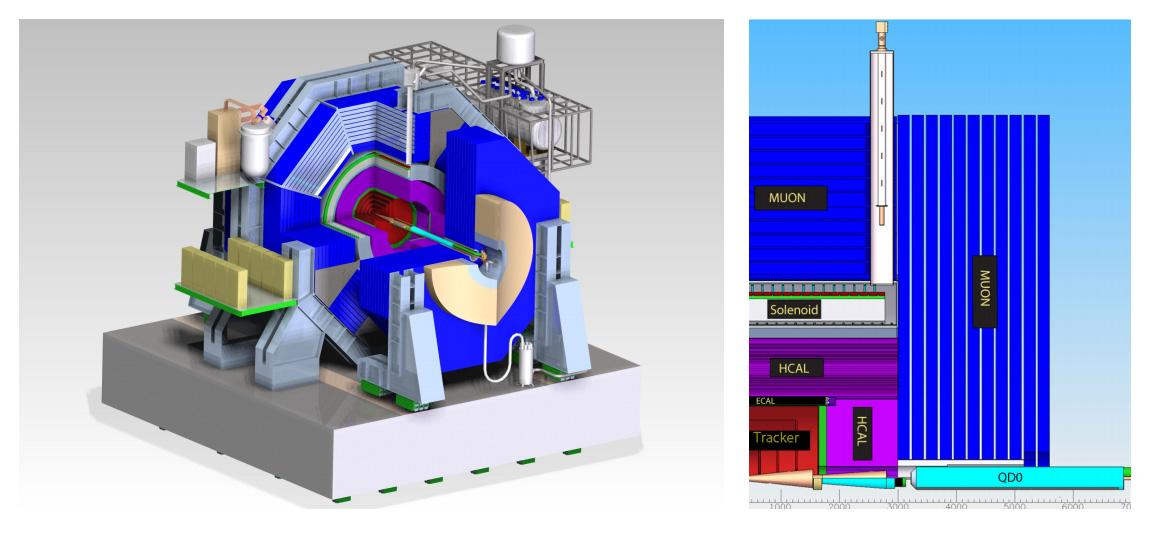
\includegraphics[width=0.95\textwidth,keepaspectratio]{Experiments/fig/SiD}
  \caption[SiD Detector]{ The Silicon Detector Concept (left). Schematic of the SiD showing the key components in a one-quarter view of a vertical section of the detector (right). \cite{ILCTDR}}
  \label{Fig:SiD}
\end{figure}

The \ac{SiD} (\reffig{Fig:SiD}) is overall quite similar to ILD with the two main differences being that SiD uses a stronger 5T magnet and a different form of tracking. Tracking at the SiD uses silicon strips rather than a TPC. This results in a better performance but is considerably more expensive. As this is the only signifcant difference from ILD we will not go into any further detail about the subdetector technologies used for SiD.

\section{Linear Collider Analysis Framework}

Before progressing further, it is useful to have a brief overview of the software used for linear collider analysis. Both \ac{ILC} and \ac{CLIC} use the same core set of packages referred to as ILCSoft. This shared framework makes it easy for work done for one experiment to be ported for use in the other which is beneficial for both experiments as it reduces the amount of work needed for each and helps prevent duplication of efforts. Here we will give an overview of the most commonly used packages in ILCSoft.

\subsection{Mokka}
Mokka is a Geant4 based simulation package available in ILCSoft. Mokka allows users to take ``.stdhep'' files created from an event generator such as PYTHIA or WHIZARD, simulates how a detector will respond in the presence of the events and outputs info such as calorimeter and tracker hits into a ``.slcio'' (the standard linear collider file format.) Standard detector geometries are stored in a database online from which Mokka extracts them at runtime. The geometry is modular in design with components such as the ECAL and TPC described separately. Users are able to customize the detector for simulation studies by replacing the standard detector components with an alternative version. The modules can even be customized manually in the Mokka steering file e.g. the number of layers in the ECAL or the thickness of the sensitive layer in the HCAL can be changed. Mokka will then automatically try to resize the customized component to make it fit in the appropriate space within the larger detector design. As well as accepting ``.stdhep'' files Mokka also has an inbuilt ``particle gun'' which can be used to fire particles with any energy at any position within the detector. This tool is particularly useful for studying a particular component of the detector without worrying about the effect of any of the components between it and the \ac{IP}.

\subsection{Pandora Particle Flow Algorithm}
\label{Pandora}
Pandora is an advanced Particle Flow Algorithm used at linear colliders which allows an increased level of precision from detector measurements by combining information from all the different detector components. The main aim of a \ac{PFA} is to associate calorimeter hits with individual tracker hits using topology then use the tracker information to calculate the particles' energy, as there is less uncertainty on this than on the measurement by the calorimeter. If there is ambiguity when associating tracks with hits (e.g. in jets) then the \ac{PFA} will instead use the calorimeter to determine the particles energy. Because we ideally want to use the track measurements for every particle the performance of the \ac{PFA} is boosted by having a high spatial resolution measurement at the end of the tracker (e.g. the \ac{SET} in \ac{ILD}) and having a high granularity calorimeter at the start of the \ac{ECAL} as this reduces the ambiguity when associating tracks with calroimeter hits. The optimization for \ac{PFA} has been one the main influencing factors for the design of the detectors at ILC and CLIC. In ILCSoft Pandora is implemented in Marlin (see below) and is used to convert the hits output by Mokka into reconstructed particles referred to as \ac{PFOs}.

\subsection{Marlin}
Marlin is the main analysis tool in ILCSoft. It is a modular framework which applies a series of processors to an event where each processor can be built separately to perform a seperate task. For example one processor might perform jet finding while another might carry out lepton finding. Marlin is controlled with xml steering files containing a list of the processors to be used, the lcio files on which Marlin will act, the detector geometry used by Mokka and the parameters which the processors need e.g.\ energy cuts or jet radius. The main benefit of the Marlin system is the ability to ``plug and play'' by which we mean processors can be added/removed and their parameters can be changed in the Marlin steering file to change the analysis at any time without having to recompile any code. Processors from one analyis can also be used in another analysis simply by including them in the steering file with the idea being that eventually there will be a large database of processors which users can pick and choose from without having to construct their own. The ILCSoft installation already comes with standard processors that link in to FastJet (jet finding), LCFIPLUS (flavour tagging), Root and Pandora.

A typical analyis from start to finish might proceed as follows:
\begin{itemize}
\item Generate event with Whizard, output is stdhep file
\item Simulate event in detector with Mokka, output is lcio file with raw detector hits
\item Apply Pandora PFA using Marlin, output is lcio file containing reconstructed particles
\item Perform Analysis using Marlin, output is Root ntuple containing parameters like missing energy, number of jets etc 
\end{itemize}



